\section{Aufgabe 6}
\setcounter{section}{6}

\begin{enumerate}[(a)]
    \item Skizzieren Sie die Menge $[-1, 3] \times \{-2,2,3\}$.

        \begin{align*}
            M = [-1, 3] \times \{-2,2,3\} &= \{-1, 0, 1, 2, 3\} \times \{-2, 2, 3\} = \\
                                          &=
                    \begin{aligned}[t]
                        \{&(-1, -2), (-1, 2), (-1, 3), (0, -2), (0, 2),\\
                          &(0, 3), (1, -2), (1, 2), (1, 3), (2, -2), (2, 2),\\
                          &(2, 3), (3, -2), (3, 2), (3, 3)\}
                    \end{aligned}
        \end{align*}

        \begin{figure}[h]
            \centering
            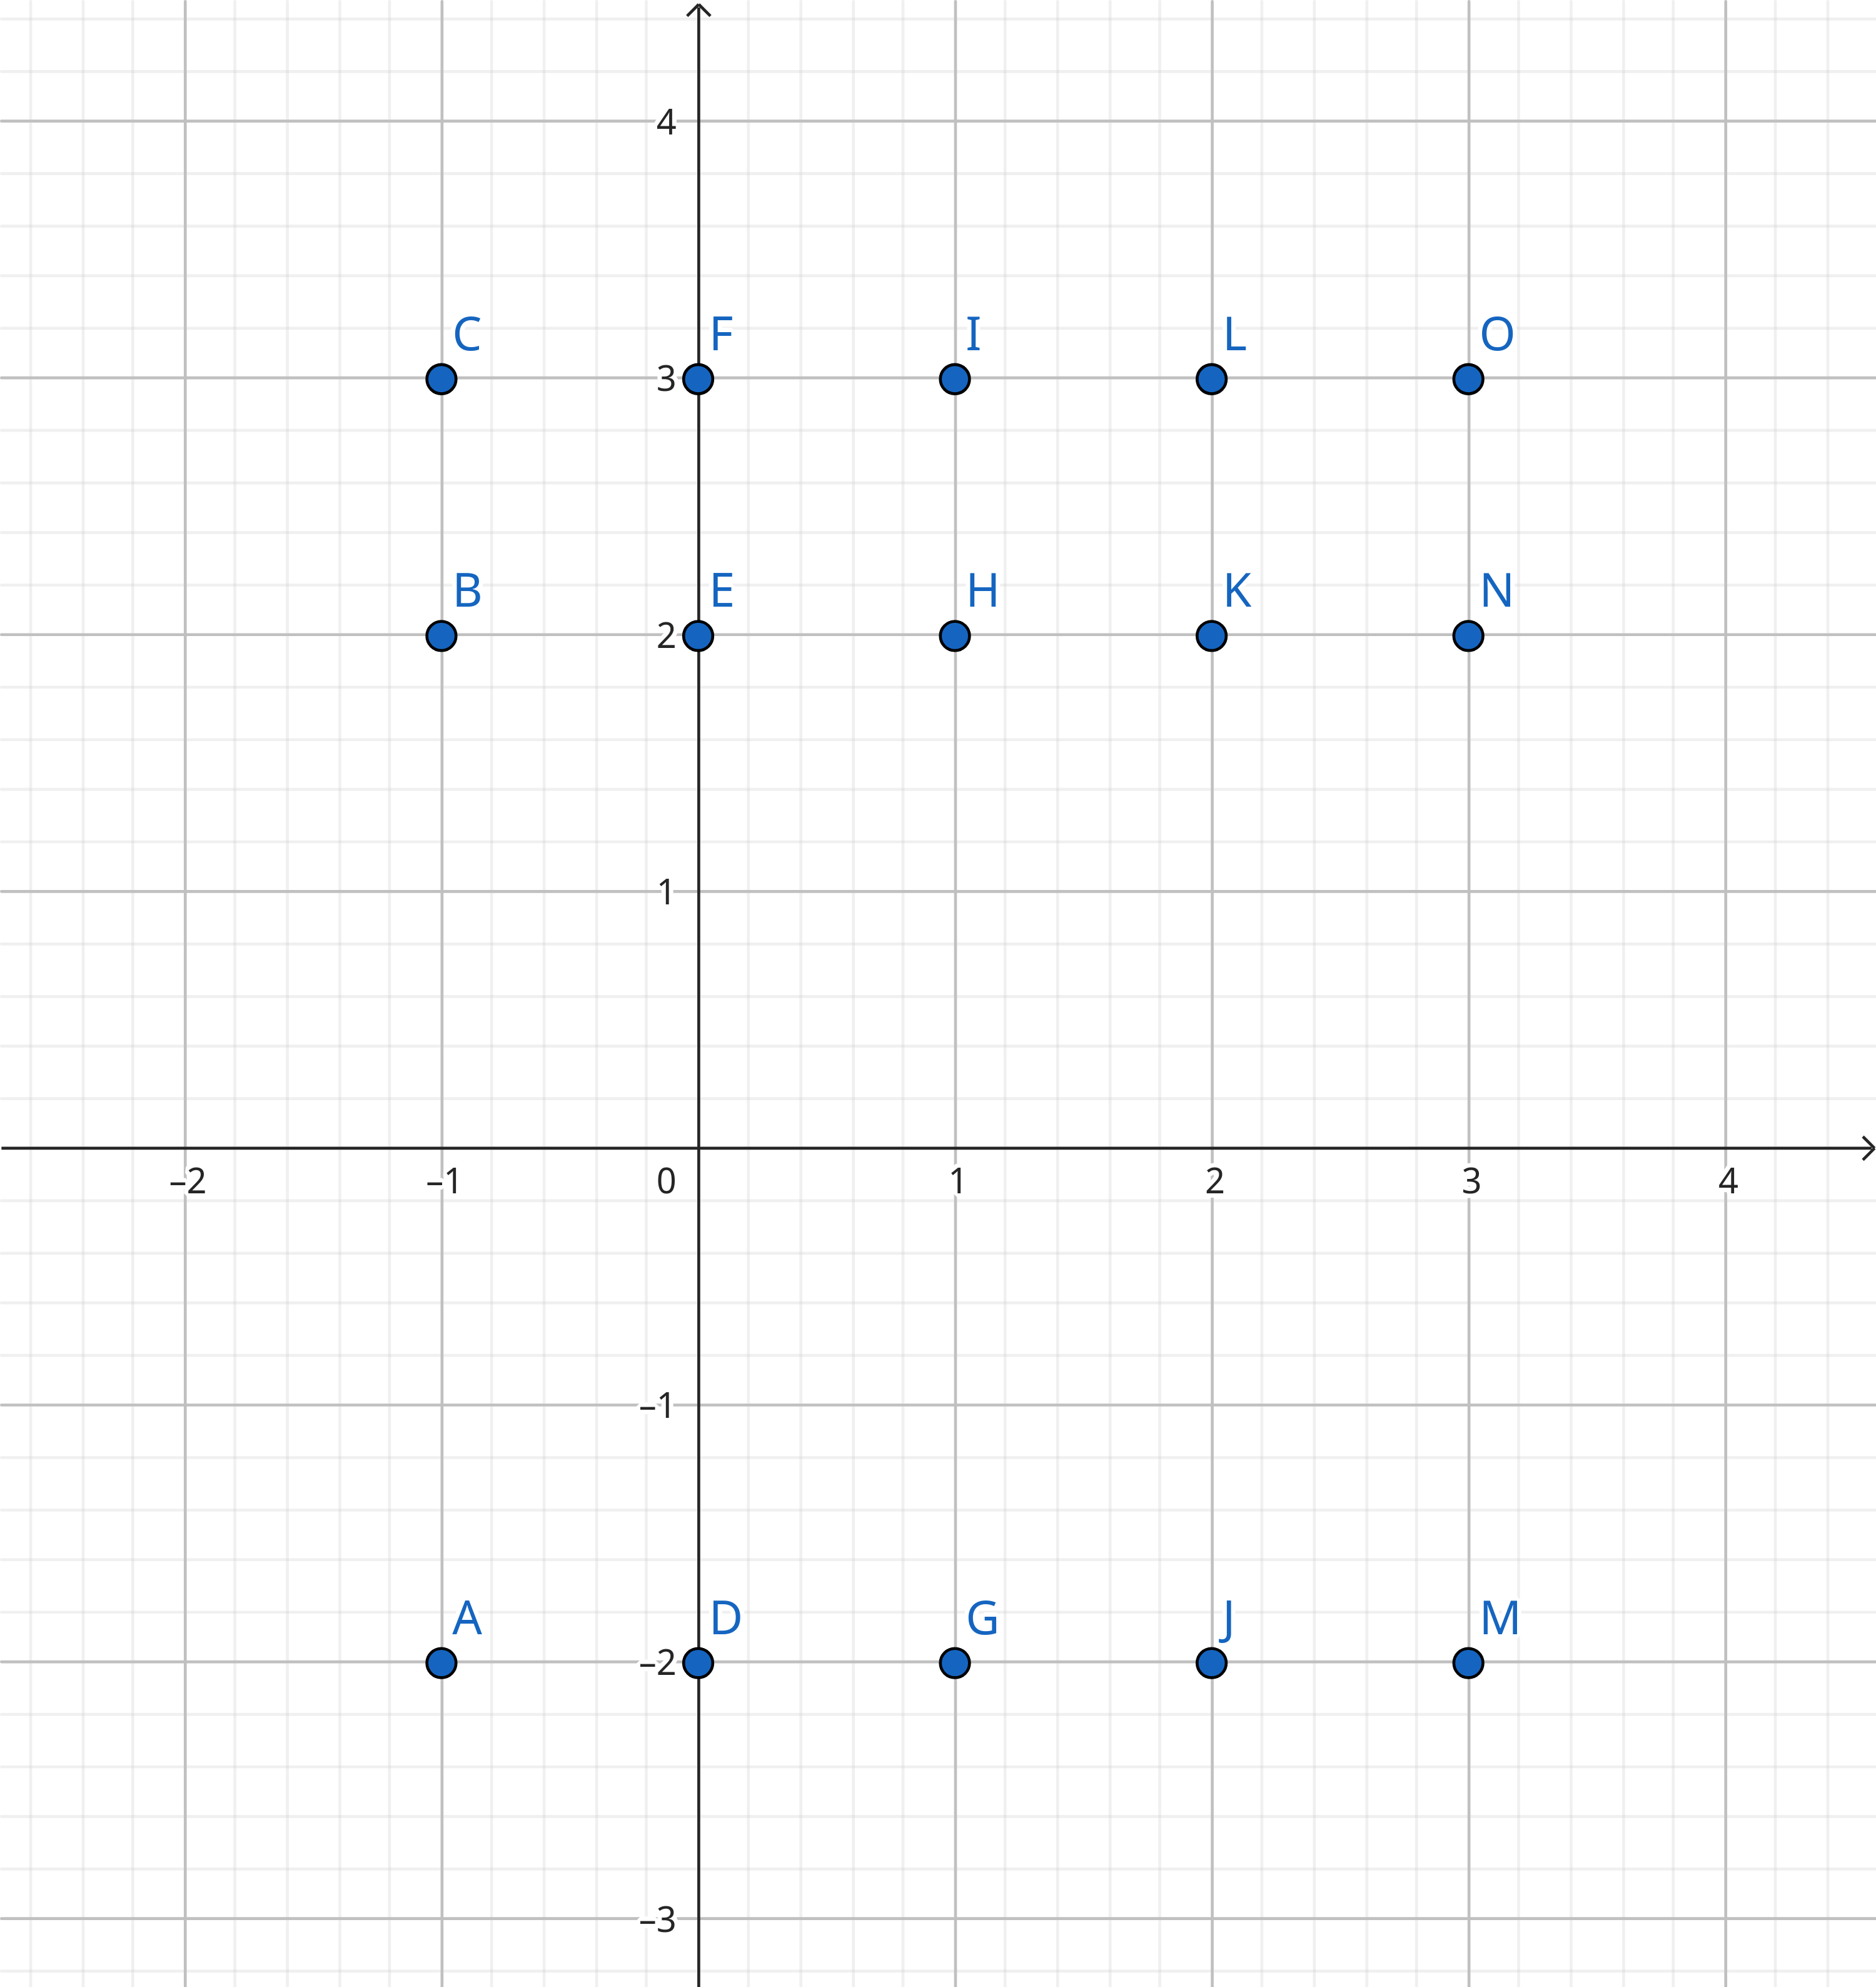
\includegraphics[width=0.55\textwidth]{./assets/abbildung-06-01.png}
            \caption{$[-1,3] \times {-2,2,3}$}
        \end{figure}

    \pagebreak

    \item Schreiben Sie folgende Menge durch Aufz"ahlen all ihrer Elemente
        $(\mathbb{Z} \times \{-1, -2\}) \cap (\{3, 4\} \times \mathbb{Z})$.

        \begin{align*}
            M &= (\mathbb{Z} \times \{-1, -2\}) \cap (\{3, 4\} \times \mathbb{Z}) =\\[5pt]
              &=
              \begin{aligned}[t]
                  \{(x_1, x_2) \text{ : }& x_1 \in \mathbb{Z} \text{, } x_2 \in \{-1, -2\} \text{ und}\\
                                         & x_1 \in \{3, 4\} \text{, } x_2 \in \mathbb{Z}\} =
              \end{aligned}\\
              &= \{(x_1, x_2) \text{ : } x_1 \in \{3, 4\} \text{, } x_2 \in \{-1, -2\}\} =\\[5pt]
              &= \{(3, -1), (3, -2), (4, -1), (4, -2)\}
        \end{align*}
\end{enumerate}

